\documentclass[11pt, oneside]{article}   	% use "amsart" instead of "article" for AMSLaTeX format
\usepackage{geometry}                		% See geometry.pdf to learn the layout options. There are lots.
\geometry{letterpaper}                   		% ... or a4paper or a5paper or ... 
%\geometry{landscape}                		% Activate for for rotated page geometry
%\usepackage[parfill]{parskip}    		% Activate to begin paragraphs with an empty line rather than an indent
\usepackage{graphicx}				% Use pdf, png, jpg, or eps� with pdflatex; use eps in DVI mode
								% TeX will automatically convert eps --> pdf in pdflatex		
\usepackage{amssymb}
\usepackage{amsmath}

\title{Pyramids and cones}
%\author{The Author}
\date{}							% Activate to display a given date or no date

\graphicspath{{/Users/telliott_admin/Dropbox/Tex/png/}}

\usepackage{listings,relsize} 
\lstloadlanguages{R} 
\lstset{language=R,basicstyle=\smaller[1],commentstyle=\rmfamily\smaller, 
  showstringspaces=false,% 
  xleftmargin=4ex,literate={<-}{{$\leftarrow$}}1 {~}{{$\sim$}}1} 
\lstset{escapeinside={(*}{*)}}   % for (*\ref{ }*) inside lstlistings (S code) 
\begin{document}

\maketitle
%\section{}
% \subsection*{R code}
% \begin{lstlisting}  \end{lstlisting}
% \begin{center} 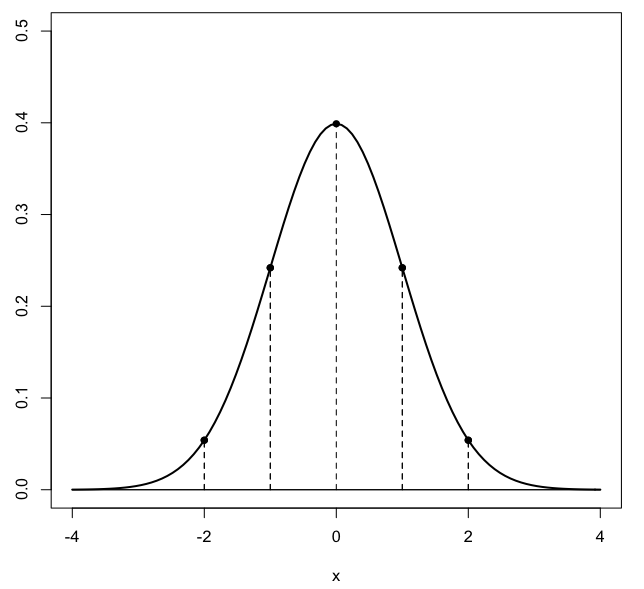
\includegraphics [scale=0.4] {gauss3.png} \end{center}
% \begin{bmatrix} a  &  b \\ c  &  d \end{bmatrix}
% \bigg |_

\large
\noindent In this short write-up I want to get a formula for the volume of a cone.  But let's start with a right pyramid.  This is a pyramid with its apex aligned directly above the center of the base.  Our example also has a square base.  Start with a cube, and find the point at its center.  
\begin{center} 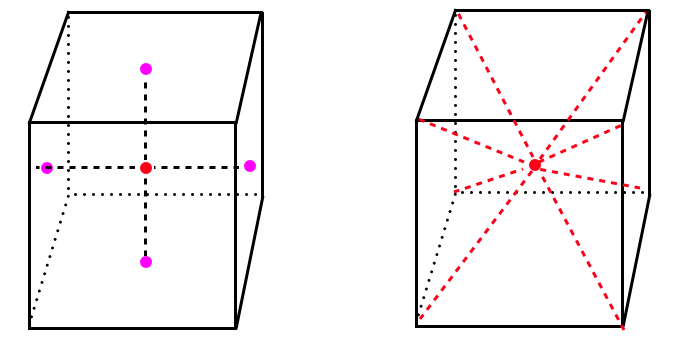
\includegraphics [scale=0.4] {cubes.png} \end{center}
Now draw  lines from the center to each of the $8$ vertices, and cut along the plane formed by each two adjacent lines and the base that connects them.  (This is easier said than done.  One way is to start by balancing the cube on one edge, then sawing straight down from the opposing edge, separating the cube in half).  By one method or another, we end up with $6$ identical right pyramids each with a square base.
\begin{center} 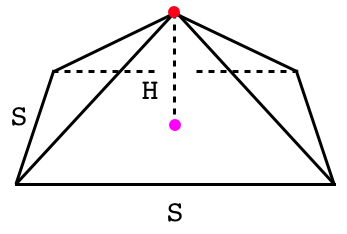
\includegraphics [scale=0.4] {sq_pyramid.png} \end{center}
If the side length of the original cube is S, then the volume of the original cube is $S^3$, now separated into $6$ identical pyramids, so the volume of each is $S^3/6$.  Since the height of each is only one-half the side length, the volume is also given by the formula
\[ V = \frac{1}{6}S^3 = \frac{1}{6}(2H)S^2 = \frac{1}{3}HS^2 \]
Note that this formula is equivalent to 
\[ V = \frac{1}{3}HA \]
where A is the area of the base.

We've shown that the formula is correct for this particular example, but we haven't shown it in general, although as it turns out it is true for all solids of this type.  

Try to think of the volume as consisting of the sum of a series of slices cut parallel to the base, and imagine what would happen to the shape of the slices if we could move the apex  off-center.  Here is a top view of such a pyramid.  The four maroon dots are the corners of the base formed by a slice about half-way down.

\begin{center} 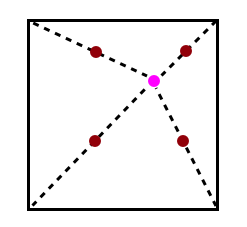
\includegraphics [scale=0.4] {top_pyramid.png} \end{center}
By using similar triangles, one can show that the shape and area of the cross-section at each height is in the same proportion to the base as the section height is to the total height.

Since the area of each section is unchanged by moving the apex, the volume should be unchanged as well.

It's a little harder to figure out what should happen if the total height changes.  And harder still to make the leap to other shapes, like a the circular cross-section for a cone.  Nevertheless, the formula above holds for any shape where the area changes as the square of the height.

Let's do things systematically.  Consider this vertical cross-section of half of a pyramid.  $X$ goes from the center point to the middle of a side.
\begin{center} 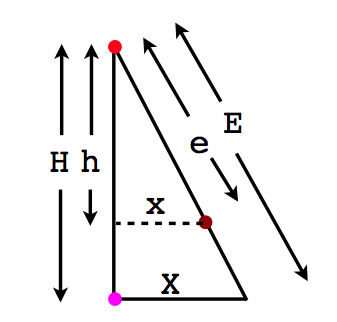
\includegraphics [scale=0.4] {sim_triangles.png} \end{center}
The total height $H$, and the distance from the central axis to the edge $X$, as well as the edge length $E$  are given, as are the corresponding values for a cross-section parallel to the base, taken at $h$, measuring down from the top.  It is clear, by similar triangles, that all these values should be in the same proportion, e.g. $x/h = X/H$.

So the cross-section cut at height $h$ has a half side length of $x$ and an area of 
\[ A = (2x)^2 = 4x^2 \]
If $\theta$ is the angle between $H$ and $E$, then
\[ x = h \ tan \ \theta, \ \ \theta = const \]
and it is clear that the area is proportional to $h^2$.  
\[ A = 4x^2 = 4(h \ tan \ \theta)^2 \]
if 
\[ k = 4 \ tan^2 \ \theta \]
\[ A = kh^2 \]

Using calculus terminology, we divide up the height into a bunch of very small intervals $dh$, look at the section or slice at each height and measure the area for each, proportional to $h^2$.  Then we compute the volume of the small slice, which is equal to the width of the slice $dh$ times the area.  Finally we add the volumes of all the little slices up by integrating
\[ V = \int_0^H kh^2 \ dh \]
This is almost the simplest integral there is and the first one you compute
\[ \int h^2 \ dh = \frac{1}{3}h^3 \]
\[  V = k \int_0^H kh^2 \ dh = \frac{1}{3}h^3 \ \bigg |_0^H = \frac{1}{3}kH^3 \]
Going back to the area of the base, it is
\[ A = 4X^2 = 4(H \ tan \ \theta)^2 = kH^2 \]
So indeed
\[  V = \frac{1}{3}kH^3 = \frac{1}{3}HA\]
In the case of a cone, with a circular cross-section, we would probably change the labels $x$ and $X$ to $r$ and $R$, but nothing else would change about the argument.  It's exactly the same, and the formula for volume of a cone is
\[  V = \frac{1}{3}HA = \frac{1}{3}H \ \pi R^2 \]


\end{document}  